\documentclass[a4paper]{article}

% Packages
\usepackage[14pt]{extsizes}
\usepackage[T2A]{fontenc}
\usepackage[russian]{babel}
\usepackage[left=20mm, top=15mm, right=15mm, bottom=20mm]{geometry}
\usepackage{graphicx} % For images
\usepackage{amsmath, amssymb} % For equations
\usepackage{booktabs} % For better tables
\usepackage{pgfplots} % For plotting graphs
\usepackage{xcolor} % For color support
\usepackage{caption} % For captioning tables and figures
\usepackage{float} % For precise float placement (images, tables)
\usepackage{array} % For better table management
\pgfplotsset{compat=1.17}

% Importing custom definitions (lstset, tikzset, etc.)
\newcommand{\labtitle}[9]{
	\begin{center}
		\vspace*{-1.8cm}
		
\includegraphics[width=0.26\textwidth]{../common/itmo-logo.png}\\
		\vspace{2.4cm}
		\textbf{\Large Основы электротехники}\\[1.2cm]
		\textbf{\Large Отчёт по лабораторной работе №#1}\\[0.7cm]
		\textbf{\Large #2}\\[3cm]

		\textbf{\Large Группа \textcolor{red}{\textit{P#3}}}\\[0.2cm]
		\textbf{\Large Вариант \textcolor{red}{\textit{#4}}}\\[3cm]

		\begin{flushleft}
			\textbf{\large Выполнил: \textcolor{red}{\textit{#5}}}\\[0.5cm]
			\textbf{\large Дата сдачи отчёта: \textcolor{red}{#6}}\\[0.5cm]
			\textbf{\large Дата защиты: \textcolor{red}{#7}}\\[0.5cm]
			\textbf{\large Контрольный срок защиты: \uline{#8}}\\[0.5cm]
			\textbf{\large Количество баллов: \uline{#9}}\\[2cm]
		\end{flushleft}
	\end{center}

	\vspace*{\fill}
	\begin{center}
		\textbf{\Large СПб -- 2024}
	\end{center}
	\vspace*{-1.8cm}
}

\newcommand{\hwtitle}[8]{
	\begin{center}
		\vspace*{-1.8cm}
		
\includegraphics[width=0.26\textwidth]{../common/itmo-logo.png}\\
		\vspace{2.4cm}
		\textbf{\Large Основы электротехники}\\[1.2cm]
		\textbf{\Large Домашнее задание №#1}\\[0.7cm]
		\textbf{\Large #2}\\[3cm]

		\textbf{\Large Группа \textcolor{red}{\textit{P#3}}}\\[0.2cm]
		\textbf{\Large Вариант \textcolor{red}{\textit{#4}}}\\[3cm]

		\begin{flushleft}
			\textbf{\large Выполнил: \textcolor{red}{\textit{#5}}}\\[0.5cm]
			\textbf{\large Дата сдачи: \textcolor{red}{#6}}\\[0.5cm]
			\textbf{\large Контрольный срок сдачи: \uline{#7}}\\[0.5cm]
			\textbf{\large Количество баллов: \uline{#8}}\\[2cm]
		\end{flushleft}
	\end{center}

	\vspace*{\fill}
	\begin{center}
		\textbf{\Large СПб -- 2024}
	\end{center}
	\vspace*{-1.8cm}
}

% % listing for programming code blocks
\lstset{
	language=C++,                 % Programming language
	basicstyle=\ttfamily\normalsize, % Adjust font size
	keywordstyle=\color{blue},    % Style for keywords
	stringstyle=\color{red},      % Style for strings
	commentstyle=\color{gray},   % Style for comments
	morecomment=[l][\color{magenta}]{\#}, % Special comment style
	breaklines=true,              % Line breaking in long lines
	numbers=left,                 % Line numbering on the left
	numberstyle=\tiny\color{gray},% Style for line numbers
	frame=single,                 % Code frame
	showstringspaces=false        % Don't show spaces in strings
}

% % tikz styles for flowcharts
\tikzset{
	startstop/.style={
			rectangle,
			rounded corners,
			minimum width=3cm,
			minimum height=1cm,
			text centered,
			draw=black,
			fill=red!30
		},
	io/.style={
			trapezium,
			trapezium left angle=70,
			trapezium right angle=110,
			minimum width=3cm,
			minimum height=1cm,
			text centered,
			draw=black,
			fill=blue!30
		},
	process/.style={
			rectangle,
			minimum width=3cm,
			minimum height=1cm,
			text centered,
			draw=black,
			fill=orange!30
		},
	decision/.style={
			diamond,
			aspect=2,
			minimum width=3cm,
			text centered,
			draw=black,
			fill=green!30
		},
	arrow/.style={
			thick,
			->,
			>=stealth
		},
	prep/.style={
			chamfered rectangle,
			chamfered rectangle xsep=2cm,
			draw,
			thick,
			minimum width=5cm,
			minimum height=1cm,
			text centered,
			text width=2.5cm,
			font=\small,
			fill=yellow!30
		},
}


\begin{document}

% Title page
\labtitle{1}{Исследование характеристик источника электрической энергии постоянного тока}{3331}{33}{Дворкин Борис Александрович}{16.09.2024}{09.10.2024}{09.10.2024}{}
\thispagestyle{empty}

\newpage
\pagestyle{plain}
\setcounter{page}{1}

% Section 1: Цель работы
\section{Цель работы}
Исследование режимов работы и экспериментальное определение параметров схемы замещения источника электрической энергии. К выполнению работы следует приступать после изучения раздела «Источники электрической энергии».

% Section 2: Схема эксперимента
\section{Схема эксперимента}
На рисунке 1.1 представлена схема замещения источника электрической энергии постоянного тока и нагрузки, созданная в приложении LTspice.

\begin{figure}[H]
	\centering
	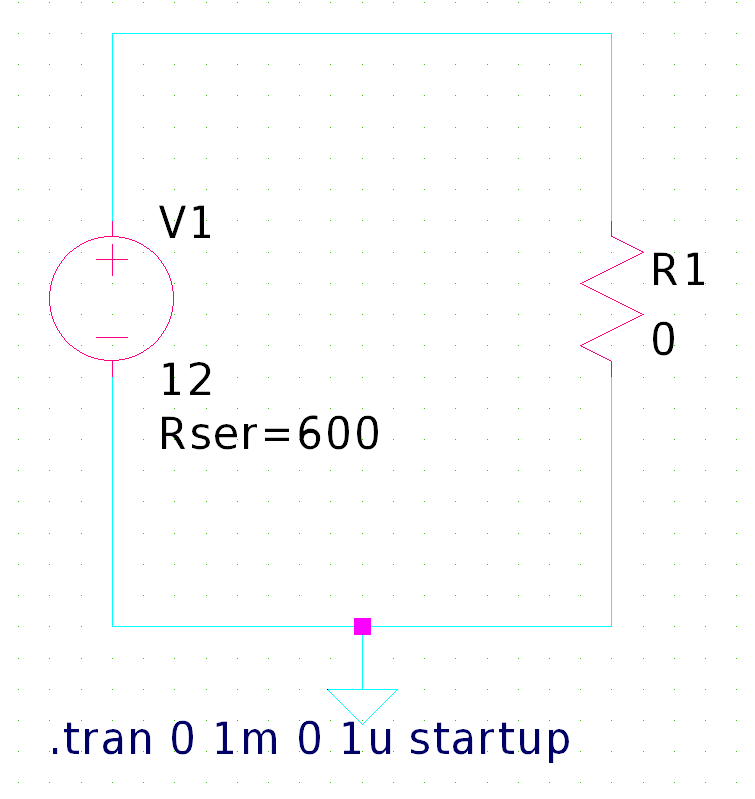
\includegraphics[width=0.6\textwidth]{schema.png} % Make sure the path to the image is correct
	\caption{Схема замещения источника электрической энергии в LTspice.}
\end{figure}

% Section 3: Расчёт значения + погрешностей; Табличка 1.1
% Section 3: Таблица измерений
\section{Заполненная таблица 1.1}

% Формулы для расчётов
\subsection{Формулы для расчёта}

Ток через нагрузку рассчитывается по формуле:
\[
	I_n = \frac{U_n}{R_n} \; \text{[А]},
\]
где \( U_n \) — измеренное напряжение на нагрузке, а \( R_n \) — сопротивление нагрузки.

Абсолютная погрешность тока:
\[
	\Delta I_n = \frac{\Delta U_n}{R_n}.
\]
, где R - известная константа, а U - измеренная величина

Внутреннее сопротивление источника для каждого промежутка между измерениями рассчитывается по формуле:
\[
	r_k = \frac{U_{n_k} - U_{n_{k+1}}}{I_{n_{k+1}} - I_{n_k}} \; \text{[Ом]}.
\]

Абсолютная погрешность внутреннего сопротивления \( \Delta r_k \):
\[
	\Delta r_k = \frac{|\Delta(U_{n_k} - U_{n_{k+1}}) \cdot (I_{n_{k+1}} - I_{n_k}) + \Delta(I_{n_{k+1}} - I_{n_k}) \cdot (U_{n_k} - U_{n_{k+1}})|}{(I_{n_{k+1}} - I_{n_k})^2}.
\]

Абсолютная погрешность разности напряжений:
\[
	\Delta(U_{n_k} - U_{n_{k+1}}) = \Delta U_{n_k} + \Delta U_{n_{k+1}}.
\]

Абсолютная погрешность разности токов:
\[
	\Delta(I_{n_{k+1}} - I_{n_k}) = \Delta I_{n_{k+1}} + \Delta I_{n_k}.
\]

Абсолютная погрешность измерения напряжения (округляем до тысячных):
\[
	\Delta U_n = \frac{\text{цена младшего разряда}}{2} = \frac{0{,}001\,\text{В}}{2} = 0{,}0005\,\text{В}.
\]

\subsection{Пример расчёта для \( k = 2 \)}

1. \textit{Вычисляем разности напряжений и их погрешности:}
\begin{align*}
	U_{n_2} - U_{n_3}         & = 10{,}800\,\text{В} - 9{,}600\,\text{В} = 1{,}200\,\text{В},                                     \\
	\Delta(U_{n_2} - U_{n_3}) & = \Delta U_{n_2} + \Delta U_{n_3} = 0{,}0005\,\text{В} + 0{,}0005\,\text{В} = 0{,}0010\,\text{В}.
\end{align*}

2. \textit{Вычисляем токи и их погрешности:}
\begin{align*}
	I_{n_2}        & = \frac{10{,}800\,\text{В}}{5400\,\Omega} = 0{,}0020\,\text{А},                     \\
	\Delta I_{n_2} & = \frac{0{,}0005\,\text{В}}{5400\,\Omega} \approx 9{,}259 \times 10^{-8}\,\text{А}, \\
	I_{n_3}        & = \frac{9{,}600\,\text{В}}{2400\,\Omega} = 0{,}0040\,\text{А},                      \\
	\Delta I_{n_3} & = \frac{0{,}0005\,\text{В}}{2400\,\Omega} \approx 2{,}083 \times 10^{-7}\,\text{А}.
\end{align*}

3. \textit{Вычисляем разности токов и их погрешности:}
\begin{align*}
	I_{n_3} - I_{n_2}         & = 0{,}0040\,\text{А} - 0{,}0020\,\text{А} = 0{,}0020\,\text{А},                                                                             \\
	\Delta(I_{n_3} - I_{n_2}) & = \Delta I_{n_3} + \Delta I_{n_2} = 2{,}083 \times 10^{-7}\,\text{А} + 9{,}259 \times 10^{-8}\,\text{А} = 3{,}009 \times 10^{-7}\,\text{А}.
\end{align*}

4. \textit{Вычисляем \( r_2 \) и его погрешность:}
\[
	r_2 = \frac{1{,}200\,\text{В}}{0{,}0020\,\text{А}} = 600{,}000\,\Omega.
\]

\[
	\Delta r_2 = \frac{|\Delta(U_{n_2} - U_{n_3}) \cdot (I_{n_3} - I_{n_2}) + \Delta(I_{n_3} - I_{n_2}) \cdot (U_{n_2} - U_{n_3})|}{(I_{n_3} - I_{n_2})^2}.
\]

Подставляем значения:
\begin{align*}
	\Delta r_2 & = \frac{|0{,}0010\,\text{В} \cdot 0{,}0020\,\text{А} + 3{,}009 \times 10^{-7}\,\text{А} \cdot 1{,}200\,\text{В}|}{(0{,}0020\,\text{А})^2}     \\
	           & = \frac{(2{,}000 \times 10^{-6}\,\text{В}\cdot\text{А} + 3{,}6108 \times 10^{-7}\,\text{В}\cdot\text{А})}{4{,}000 \times 10^{-6}\,\text{А}^2} \\
	           & = \frac{2{,}3611 \times 10^{-6}\,\text{В}\cdot\text{А}}{4{,}000 \times 10^{-6}\,\text{А}^2} = 0{,}5903\,\Omega \approx 0{,}590\,\Omega.
\end{align*}

\subsection{Результаты расчётов}

Проводим аналогичные расчёты для всех \( k \) от 2 до 10 и получаем:

\begin{table}[H]
	\centering
	\caption*{Значения \( r_k \) и их абсолютные погрешности \( \Delta r_k \)}
	\begin{tabular}{|c|c|c|}
		\hline
		\( k \) & \( r_k \), Ом & \( \Delta r_k \), Ом \\
		\hline
		2       & 600{,}000     & \( \pm \) 0{,}590    \\
		3       & 600{,}000     & \( \pm \) 0{,}670    \\
		4       & 600{,}000     & \( \pm \) 0{,}774    \\
		5       & 600{,}000     & \( \pm \) 0{,}917    \\
		6       & 600{,}000     & \( \pm \) 1{,}125    \\
		7       & 599{,}301     & \( \pm \) 1{,}455    \\
		8       & 600{,}701     & \( \pm \) 2{,}090    \\
		9       & 602{,}015     & \( \pm \) 3{,}778    \\
		10      & 598{,}015     & \( \pm \) 2{,}711    \\
		\hline
	\end{tabular}
\end{table}

\subsection{Вычисление значения внутреннего сопротивления и его погрешности}

Среднее квадратическое значение внутреннего сопротивления:
\[
	\begin{aligned}
		r & = \sqrt{\frac{\sum\limits_{k=2}^{10} r_k^2}{9}}                                                           \\
		  & = \sqrt{\frac{(600{,}000)^2 \times 5 + (599{,}301)^2 + (600{,}701)^2 + (602{,}015)^2 + (598{,}015)^2}{9}} \\
		  & = 600{,}004\,\Omega.
	\end{aligned}
\]

Абсолютная погрешность \( \Delta r \) вычисляется как среднеквадратическое из погрешностей \( \Delta r_k \):
\[
	\Delta r = \sqrt{\frac{\sum_{k=2}^{10} (\Delta r_k)^2}{9}}.
\]

Подставляем значения:
\[
	\begin{aligned}
		\sum_{k=2}^{10} (\Delta r_k)^2 & = (0{,}59)^2 + (0{,}67)^2 + (0{,}774)^2 + (0{,}917)^2 + (1{,}125)^2 \\
		                               & \quad + (1{,}455)^2 + (2{,}09)^2 + (3{,}778)^2 + (2{,}711)^2        \\
		                               & = 0{,}3481 + 0{,}4489 + 0{,}599076 + 0{,}840889 + 1{,}265625        \\
		                               & \quad + 2{,}117025 + 4{,}3681 + 14{,}273284 + 7{,}349521            \\
		                               & = 31{,}6105.
	\end{aligned}
\]

Тогда:
\[
	\Delta r = \sqrt{\frac{31{,}6105}{9}} = \sqrt{3{,}5123} = 1{,}874\,\Omega.
\]

\subsection{Вычисление тока короткого замыкания и его погрешности}

Ток короткого замыкания:
\[
	I_{sc} = \frac{E}{r} = \frac{12{,}000\,\text{В}}{600{,}004\,\Omega} \approx 20{,}000\,\text{мА}.
\]

Абсолютная погрешность \( \Delta I_{sc} \):
\[
	\Delta I_{sc} = I_{sc} \left( \frac{\Delta E}{E} + \frac{\Delta r}{r} \right).
\]

Абсолютная погрешность ЭДС:
\[
	\Delta E = \frac{0{,}001\,\text{В}}{2} = 0{,}0005\,\text{В}.
\]

Вычисляем:
\[
	\Delta I_{sc} = 20{,}000\,\text{мА} \left( \frac{0{,}0005\,\text{В}}{12{,}000\,\text{В}} + \frac{1{,}189\,\Omega}{600{,}004\,\Omega} \right) \approx 0{,}040\,\text{мА}.
\]

Итоговое значение:
\[
	I_{sc} = (20{,}000 \pm 0{,}040)\,\text{мА}.
\]

\subsection{Результат}

Среднее внутреннее сопротивление:
\[
	r = (600{,}004 \pm 1{,}874)\,\Omega.
\]

Ток короткого замыкания:
\[
	I_{sc} = (20{,}000 \pm 0{,}040)\,\text{мА}.
\]

Экспериментальные значения совпадают с расчётными в пределах погрешности, что подтверждает корректность проведённых измерений и расчётов.


% Section 2: Таблица измерений
\subsection{Заполненная таблица 1.1}

\begin{table}[H]
	\centering
	\addtocounter{table}{0}
	\caption*{Таблица 1.1: Результаты измерений и расчётов}
	\begin{tabular}{|c|c|c|c|c|c|c|}
		\hline
		k  & \multicolumn{2}{c|}{Измерения} & \multicolumn{4}{c|}{Расчёт: r = 600.004 [Ом], E = 12 [B], Isc = 20 [мА]}                                               \\
		\hline
		0  & $R_n$ [Ом] & $U_n$ [В] & $I_n$ [мА] & $P_n$ [Вт] & $\eta$ & $r$ [Ом] \\
		\hline
		1  & $\infty$   & 12.000    & 0.00       & 0.00       & 1.0    & --       \\
		2  & 5400       & 10.800    & 2.00       & 0.022      & 0.9    & 600.00   \\
		3  & 2400       & 9.600     & 4.00       & 0.038      & 0.8    & 600.00   \\
		4  & 1400       & 8.400     & 6.00       & 0.050      & 0.7    & 600.00   \\
		5  & 900        & 7.200     & 8.00       & 0.058      & 0.6    & 600.00   \\
		6  & 600        & 6.000     & 10.00      & 0.060      & 0.5    & 600.00   \\
		7  & 400        & 4.800     & 12.00      & 0.058      & 0.4    & 599.301  \\
		8  & 257        & 3.599     & 14.004     & 0.050      & 0.3    & 600.701  \\
		9  & 150        & 2.400     & 16.00      & 0.038      & 0.2    & 602.015  \\
		10 & 67         & 1.205     & 17.985     & 0.022      & 0.1    & 598.015  \\
		11 & 0          & 0.000     & 20.00      & 0.000      & 0.0    & --       \\
		\hline
	\end{tabular}
\end{table}


% Section 3: Пример расчёта
\newpage
\section{Пример расчёта для одной строки таблицы}

Для расчёта параметров используем следующие формулы:

\begin{itemize}
	\item Ток через нагрузку:
	      \[
		      I_n = \frac{U_n}{R_n}
	      \]

	\item Мощность, рассеиваемая на нагрузке:
	      \[
		      P_n = \frac{U_n^2}{R_n}
	      \]

	\item Коэффициент полезного действия:
	      \[
		      \eta_n = \frac{R_n}{R_n + r}
	      \]

	\item Внутреннее сопротивление источника:
	      \[
		      r_k = \frac{U_k - U_{k+1}}{I_{k+1} - I_k}
	      \]
\end{itemize}

Рассчитаем значения для строки \(n = 2\):

\begin{align*}
	I_2    & = \frac{U_2}{R_2} = \frac{10.8}{5400} = 2.00 \, \text{мА},                           \\
	P_2    & = \frac{U_2^2}{R_2} = \frac{10.8^2}{5400} \approx 0.038 \, \text{Вт},                \\
	\eta_2 & = \frac{R_2}{R_2 + r} = \frac{5400}{5400 + 600} = 0.9,                                 \\
	r_2    & = \frac{U_2 - U_3}{I_3 - I_2} = \frac{10.8 - 9.6}{4 - 2} = 600 \, \text{Ом}.
\end{align*}

Таким образом, для строки \(n = 2\) были рассчитаны следующие значения:
\[
	I_2 = 2.00 \, \text{мА}, \quad P_2 = 0.038 \, \text{Вт}, \quad \eta_2 = 0.9, \quad r_2 = 600 \, \text{Ом}.
\]


% Section 4: Расчётная внешняя характеристика источника
\newpage
\section{Расчётная внешняя характеристика источника}

На рисунке \ref{fig:characteristic} представлена расчётная и экспериментальная внешняя характеристика источника.
Расчётная характеристика изображена в виде синей линии,
которая соединяет точки \((0, E = 12 \, \text{В})\) и \((I_{sc} = 20 \, \text{мА}, 0)\).
Эта линия отражает теоретическую зависимость напряжения на нагрузке \(U_n\) от тока \(I_n\),
поступающего от источника, при идеальных условиях.

Экспериментальные точки, отмеченные на графике красными квадратами,
соответствуют измеренным значениям напряжения \(U_n\) для разных токов \(I_n\),
согласно данным из таблицы 1.1. Эти точки показывают реальные данные,
полученные при изменении сопротивления нагрузки, и их отклонения от расчётной линии
могут свидетельствовать о наличии потерь или неточностей в измерениях и/или вычислениях.

\begin{figure}[h]
	\centering
	\begin{tikzpicture}
		\begin{axis}[
				width=17cm, height=14cm, % Размер графика
				xlabel={$I_n$ [мА]}, % Ось X
				ylabel={$U_n$ [В]},  % Ось Y
				axis lines=middle,
				grid=major,          % Основная сетка
				xmin=0, xmax=22,     % Диапазон по оси X
				ymin=0, ymax=13,     % Диапазон по оси Y
				domain=0:20,         % Область построения
				thick,               % Толщина линии
				legend style={at={(0.95,0.95)}, anchor=north east}, % Легенда
				label style={font=\small},
				tick label style={font=\small},
				xtick={0, 2.5, 5, 7.5, 10, 12.5, 15, 17.5, 20}, % Подписи по оси X
				ytick={0, 1, 2, 3, 4, 5, 6, 7, 8, 9, 10, 11, 12}, % Подписи по оси Y
			]

			% Линия расчетной характеристики
			\addplot[color=blue, thick] coordinates {
					(0,12) (20,0)
				};
			\addlegendentry{Расчётная характеристика}

			% Экспериментальные точки
			\addplot[color=red, only marks, mark=square*] coordinates {
					(0,12)
					(2.00, 10.8)
					(4.00, 9.6)
					(6.00, 8.4)
					(8, 7.2)
					(10, 6)
					(12.00, 4.8)
					(14.004, 3.599)
					(16, 2.4)
					(17.985, 1.2)
					(20, 0)
				};
			\addlegendentry{Экспериментальные точки}

		\end{axis}
	\end{tikzpicture}
	\caption{График расчётной и экспериментальной внешней характеристики источника}
	\label{fig:characteristic}
\end{figure}


% Section 5: Графики зависимости Pn(In) и η(In)
% \section{Графики зависимости $P_n(I_n)$ и $\eta(I_n)$}
\subsection{График зависимости мощности в нагрузке \( P_n(I_n) \)}

На рисунке 3 представлена зависимость мощности в нагрузке \( P_n \) от тока \( I_n \).
Мощность в нагрузке \( P_n \) растёт с увеличением тока \( I_n \) до определённого предела,
после чего начинает снижаться, что объясняется возрастанием сопротивления нагрузки
и уменьшением напряжения на ней.

\begin{figure}[h]
	\centering
	\begin{tikzpicture}
		\begin{axis}[
			width=17cm, height=13cm, % Размер графика
			xlabel={$I_n$~[мА]}, % Ось X
			ylabel={$P_n$~[Вт]},  % Ось Y
			axis lines=middle,
			grid=major,          % Основная сетка
			xmin=0, xmax=22,     % Диапазон по оси X
			ymin=0, ymax=0.06,   % Диапазон по оси Y
			thick,               % Толщина линии
			% scaled ticks=false,
			legend style={at={(0.95,0.95)}, anchor=north east}, % Легенда
			label style={font=\small},
			tick label style={font=\small},
			xtick={0, 2.5, 5, 7.5, 10, 12.5, 15, 17.5, 20}, % Подписи по оси X
			ytick={0, 0.01, 0.02, 0.03, 0.04, 0.05, 0.06}, % Подписи по оси Y
			]

			% Зависимость мощности P_n от I_n
			\addplot[color=blue, thick, mark=*] coordinates {
					(0, 0.00)
					(1.98, 0.021)
					(3.96, 0.038)
					(5.94, 0.049)
					(7.92, 0.056)
					(9.9, 0.059)
					(11.88, 0.056)
					(13.864, 0.049)
					(15.84, 0.038)
					(17.806, 0.021)
					(20, 0.000)
				};
			\addlegendentry{Мощность \( P_n(I_n) \)}

		\end{axis}
	\end{tikzpicture}
	\caption{График зависимости мощности в нагрузке \( P_n(I_n) \)}
\end{figure}

% \subsection{График зависимости КПД \( \eta(I_n) \)}

На рисунке 4 представлена зависимость КПД \( \eta \) от тока \( I_n \).
КПД \( \eta \) уменьшается по мере увеличения тока, 
так как больше энергии теряется внутри самого источника из-за его внутреннего сопротивления. 
Это снижает количество энергии, которое передаётся на нагрузку.

\begin{figure}[t!]
	\centering
	\begin{tikzpicture}
		\begin{axis}[
				width=17cm, height=13cm, % Размер графика
				xlabel={$I_n$ [мА]}, % Ось X
				ylabel={$\eta$},  % Ось Y
				axis lines=middle,
				grid=major,          % Основная сетка
				xmin=0, xmax=22,     % Диапазон по оси X
				ymin=0, ymax=1.1,    % Диапазон по оси Y
				thick,               % Толщина линии
				legend style={at={(0.95,0.95)}, anchor=north east}, % Легенда
				label style={font=\small},
				tick label style={font=\small},
				xtick={0, 2.5, 5, 7.5, 10, 12.5, 15, 17.5, 20}, % Подписи по оси X
				ytick={0, 0.1, 0.2, 0.3, 0.4, 0.5, 0.6, 0.7, 0.8, 0.9, 1.0}, % Подписи по оси Y
			]

			% Зависимость КПД eta от I_n
			\addplot[color=red, thick, mark=*] coordinates {
					(0, 1.0)
					(1.98, 0.9)
					(3.96, 0.8)
					(5.94, 0.7)
					(7.92, 0.6)
					(9.9, 0.5)
					(11.88, 0.4)
					(13.864, 0.3)
					(15.84, 0.2)
					(17.806, 0.1)
					(20, 0.0)
				};
			\addlegendentry{КПД \( \eta(I_n) \)}

		\end{axis}
	\end{tikzpicture}
	\caption{График зависимости КПД \( \eta(I_n) \)}
\end{figure}

\section{Графики зависимости $P_n(I_n)$ и $\eta(I_n)$}

На рисунке 3 представлена зависимость мощности в нагрузке \( P_n \) и КПД \( \eta \) от тока \( I_n \).

Мощность $P_n$ растёт с увеличением $I_n$ до определённого предела, после чего начинает снижаться из-за значительного падения напряжения на нагрузке, вызванного потерями на внутреннем сопротивлении источника.

КПД $\eta$ падает с увеличением тока $I_n$, так как больше энергии рассеивается на внутреннем сопротивлении источника (по закону Джоуля-Ленца), и меньше передаётся на нагрузку.

\begin{figure}[h]
	\centering
	\begin{tikzpicture}
		\begin{axis}[
			width=17cm, height=13cm, % Размер графика
			xlabel={$I_n$~[мА]}, % Ось X
			ylabel={$P_n$~[Вт]},  % Ось Y для мощности
			axis lines=left,
			grid=major,          % Основная сетка
			xmin=0, xmax=22,     % Диапазон по оси X
			ymin=0, ymax=0.06,   % Диапазон по оси Y для мощности
			thick,               % Толщина линии
			legend style={at={(0.95,0.85)}, anchor=north east}, % Легенда
			label style={font=\small},
			tick label style={font=\small},
			xtick={0, 2.5, 5, 7.5, 10, 12.5, 15, 17.5, 20}, % Подписи по оси X
			ytick={0, 0.01, 0.02, 0.03, 0.04, 0.05, 0.06}, % Подписи по оси Y для мощности
			]

			% Зависимость мощности P_n от I_n
			\addplot[color=blue, thick, mark=*] coordinates {
					(0, 0.00)
					(2.00, 0.022)
					(4.00, 0.038)
					(6.00, 0.050)
					(8.00, 0.058)
					(10.00, 0.060)
					(12.00, 0.058)
					(14.004, 0.050)
					(16.00, 0.038)
					(17.985, 0.022)
					(20, 0.000)
				};
			\addlegendentry{Мощность \( P_n(I_n) \)}
		\end{axis}

		% Вторая ось Y для КПД
		\begin{axis}[
			width=17cm, height=13cm, % Размер графика
			xlabel={$I_n$~[мА]}, % Ось X
			ylabel={$\eta$},  % Ось Y для КПД
			axis y line=right,
			axis x line=none,
			grid=major,          % Основная сетка
			xmin=0, xmax=22,     % Диапазон по оси X
			ymin=0, ymax=1.1,    % Диапазон по оси Y для КПД
			thick,               % Толщина линии
			legend style={at={(0.95,0.95)}, anchor=north east}, % Легенда
			label style={font=\small},
			tick label style={font=\small},
			ytick={0, 0.1, 0.2, 0.3, 0.4, 0.5, 0.6, 0.7, 0.8, 0.9, 1.0}, % Подписи по оси Y для КПД
			]

			% Зависимость КПД eta от I_n
			\addplot[color=red, thick, mark=*] coordinates {
					(0, 1.0)
					(2.00, 0.9)
					(4.00, 0.8)
					(6.00, 0.7)
					(8.00, 0.6)
					(10.00, 0.5)
					(12.00, 0.4)
					(14.004, 0.3)
					(16.00, 0.2)
					(17.985, 0.1)
					(20, 0.0)
				};
			\addlegendentry{КПД \( \eta(I_n) \)}

		\end{axis}
	\end{tikzpicture}
	\caption{Графики зависимости мощности \( P_n(I_n) \) и КПД \( \eta(I_n) \)}
\end{figure}


% Section 6: Выводы по работе
\section{Выводы по работе}

В ходе данной лабораторной работы я исследовал внешнюю характеристику источника электрической
энергии постоянного тока и определил параметры схемы его замещения, такие как внутреннее сопротивление и эдс источника, а также ток короткого замыкания. Схема была собрана в программном обеспечении для моделирования аналоговых электронных
схем «LTspice», где я измерил напряжение в цепи при различных сопротивлениях нагрузки
и выявил, что с уменьшением сопротивления нагрузки напряжение на ней падает,
а ток в цепи увеличивается. Это изменение существенно влияет на распределение мощности в
нагрузке и на эффективность работы источника.

В процессе работы я применил закон Джоуля-Ленца,
который объясняет потери мощности на внутреннем сопротивлении источника при протекании тока.
Согласно закону, выделяемая энергия на внутреннем сопротивлении источника определяется
выражением \(Q = I^2 R t\). Увеличение тока приводит к большему выделению тепла внутри источника,
что снижает количество энергии, передаваемой на нагрузку, и соответственно уменьшает КПД.

Я провёл измерение напряжения холостого хода \( U_0 \),
которое использовалось для расчёта тока короткого замыкания
и определения внешней характеристики источника.
Также я рассчитал токи, мощности и КПД на основе измерений,
что позволило оценить внутреннее сопротивление источника.
Все расчёты были проведены в Excel, где я составил таблицы с данными, а графики зависимостей
\( P_n(I_n) \) и \( \eta(I_n) \) были построены в LaTeX.
Это позволило оформить результаты в соответствии с научными стандартами и
закрепить навыки работы с математическими пакетами для дальнейшей работы,
включая подготовку к диплому.

Расчёты показали, что экспериментальное значение внутреннего сопротивления \(r = (600{,}004 \pm 1{,}874) \Omega \) совпадает с расчётным значением \( r_{\text{расч}} = 600{,}000\,\Omega \) в пределах погрешности измерений. Относительная погрешность, обусловленная округлением величин и накопленной ошибкой вычислений, \varepsilon = \(0{,}31\%\) < 1\%\, что свидетельствует о высокой точности эксперимента.

Ток короткого замыкания, рассчитанный на основе экспериментальных данных, \(I_{sc} = (20{,}000 \pm 0{,}040)\,\text{мА}\), также соответствует теоретическому значению в 20 мА. Относительная погрешность, обусловленная округлением измерений ЭДС и погрешностью эксперементально полученной величины r, составила \varepsilon = \(0{,}20\%\) < 1\%\, что также означает что эксперимент получился достаточно точный.

Эти параметры позволяют точно оценить характеристики реальной цепи.

В итоге, я пришёл к выводу, что внутреннее сопротивление источника играет критическую роль
в его характеристиках: при высоких токах оно значительно снижает эффективность передачи
энергии на нагрузку, что приводит к уменьшению КПД и снижению мощности.
Эксперимент подтвердил теоретические модели, а полученные данные дали возможность точно
рассчитать параметры реальных электрических цепей.

\end{document}
